\documentclass{article}
\usepackage{amsmath}
\usepackage{amsfonts}
\usepackage{amssymb}
\usepackage{mathdots}
\usepackage{placeins}
\usepackage{relsize,mathtools}
\usepackage{ifthen}
\usepackage{mleftright}
\usepackage{titlesec}
\usepackage{graphicx}
\usepackage{hyperref}
\usepackage[bf]{caption} % For more control over figure captions
\usepackage{subcaption}
\usepackage{listings}
\usepackage{cancel} % term cancellations in math mode
\usepackage{empheq}
\usepackage{tikz} % for drawing vector graphics
\usepackage{float}
\captionsetup{width=\textwidth}
\counterwithin{figure}{section}
\usetikzlibrary{positioning}
\usetikzlibrary{arrows.meta}
\usepackage[top=0.7in, bottom=1in, left=1in, right=1in]{geometry}

\newcommand\E[1]{\left\langle #1 \right\rangle}
\renewcommand{\d}{\mathrm{d}}
\renewcommand\Pr[1]{\begingroup
    \renewcommand\mid{\;|\;}
    \text{P({\larger[2]$\scriptstyle#1$})}
    \endgroup}
\numberwithin{equation}{section}
\hypersetup{
	colorlinks=true,
	linkcolor=blue,
	filecolor=blue,
	urlcolor=blue,
	citecolor=black
}

\begin{document}
\title{Effects of overkill and regeneration on damage output rate in Oldschool Runescape}
\author{Nukelawe}
\date{\today}
\maketitle
\section{Introduction}\label{chap:introduction}
\section{Introduction}
Efficient combat training in Oldschool Runescape is a problem of maximizing the damage output rate of the player (often measured by DPS). To optimize the DPS it is important to be able to determine its value also theoretically. Overkill and hitpoint regeneration are two major factors that have significant effects on DPS, yet the quantitative understanding of them is limited.
While simulations provide quite good results, a more mathematical viewpoint can give further insight into the nature of these effects and result in some convenient approximations.

Overkill is an effect that occurs when the damage roll exceeds the remaining hitpoints of the enemy. It is important in combat training when the idle time between kills is short, and especially when the max hit is large relative to the enemy hitpoints.

The other mechanic that will be studied is health regeneration. Assuming no regeneration is a fair approximation when regeneration rate is much slower than the damage rate. But there are inevitably scenarios where this is not the case. Whereas overkill is most significant for high damage rates, regeneration affects mostly the slower fights. While there are many ways to regain health, we will be focusing on \textit{natural regeneration} only.


\section{Fight mechanics}\label{chap:fightMechanics}
A fight consists of two parties, the attacker and the enemy. We only consider the damage dealt by the attacker on the enemy and not vice versa. In our model the enemy is attacked periodically until its remaining hitpoints are 0. The attack rate is characterized by the \textit{attack period} $T_A$ which varies between weapons.
Once every attack period the enemy is hit and the damage dealt is calulated as follows.
\begin{enumerate}
	\item The game determines if the hit will succeed by some random process which depends on various parameters, such as defensive bonuses of the enemy, offensive bonuses of the attacker and appropriate combat-related stats. We ignore the details of this process and just say the probability of the hit being successful is $a$ calling it the \textit{accuracy}. If the accuracy check fails, the attack is considered a miss and 0 damage is dealt.
	\item If the accuracy check is successful damage roll $M$, a uniformly distributed random integer between 0 and $m$ is chosen, where $m$ is the \textit{maximum hit}. Again, we do not concern ourselves with the specifics of how the max hit is determined. Notice that it is possible for the hit to deal no damage even if the accuracy check succeeds because the damage roll $M$ could be 0.
    \item If $M > H$, where $H$ is the remaining hitpoints of the enemy, the damage is capped to $H$ and the final damage dealt is $\min(M,H)$. This is the overkill effect.
\end{enumerate}

Unlike the damage calculation process, regeneration is not fundamentally random. It happens by periodically incrementing the remaining hitpoints by one until they are full. The period $T_R$ of this healing cycle is called the \emph{regeneration period} and can vary between enemies giving rise to different regeneration rates. At the beginning of a fight the state of the healing cycle can be assumed to be unknown and thus treated as a random variable. This way only the timing of the first heal is random and the rest are perfectly periodic.


\section{No regeneration}\label{chap:noregen}
\subsection{Fight model}\label{chap:fightModel}
We define the \textit{state space} as the set of all possible values the remaining hitpoints of the enemy can have during a fight. For a fight against an enemy with $h$ maximum hitpoints the state space is $\{0,\ldots,h\}$. Each hit corresponds to a transition from one state to another in the state space. The probability of transitioning to state $i$ from state $j$ is called the \textit{transition probability} and is defined as
\begin{align}\label{eq:transitionProbabilities}
    p_{ij} = \Pr{H_k = i \mid H_{k-1} = j}.
\end{align}

Let $H_k$ be the number of hitpoints the enemy has remaining after $k$ hits. A fight can be labeled with a sequence of visited hitpoint states $(H_k)_{k=0}^{n}$. For the sequence to constitute a valid $n$-hit fight we must have $H_n=0$ (fight ends in death) and $h \geq H_k > 0$ for $k<n$ (death does not happen before the last hit). As an example consider a 4-hitpoint enemy that the attacker hits 3 times, first 1, then 0 and finally 3 damage killing the enemy. This fight would be described by the sequence $4,3,3,0$ and corresponds to the highlighted path in the state space diagram in Figure~\ref{fig:stateSpace}.
\begin{figure}[h]
    \centering
    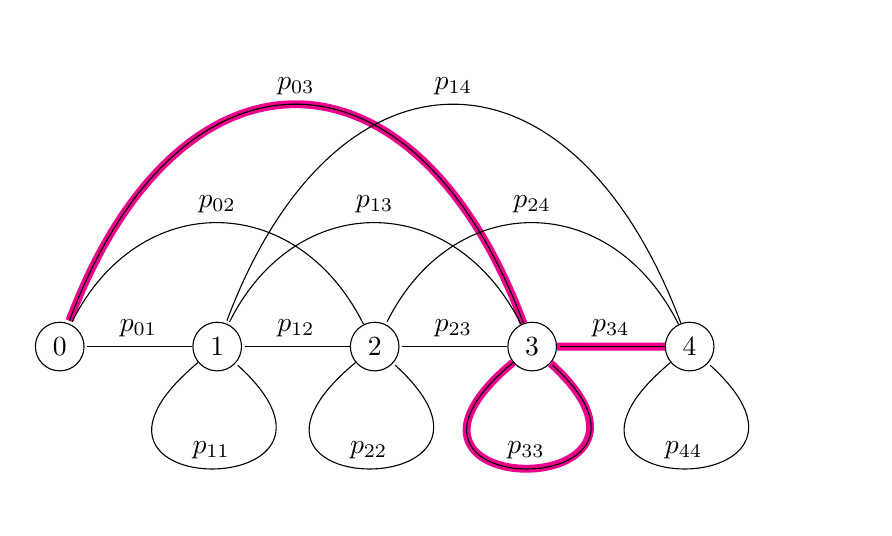
\begin{tikzpicture}[shorten >=1pt,node distance=1cm]
        \tikzstyle{state}=[shape=circle,draw,minimum size=1cm];
        \coordinate (n0);
        \xdef\scale{2}
        \xdef\maxhit{3}
        \foreach \s in {0,1,2,3,4} {
            \node[shape=circle,draw](n\s) at (\scale*\s,0){$\s$};
        }
		\path[draw, color=magenta, line width=1mm] (n4) ..
		controls({(0.75*4+0.25*3)*\scale},{2*(4-3-1)}) and ({(0.25*4+0.75*3)*\scale},{2*(4-3-1)})
		.. (n3) ..
        controls({(3-1.2)*\scale},-2) and ({(3+1.1)*\scale},-2)
		.. (n3) ..
		controls({(0.75*3+0.25*0)*\scale},{2*(3-0-1)}) and ({(0.25*3+0.75*0)*\scale},{2*(3-0-1)})
		.. (n0);
        \foreach \from in {1,2,3,4} {
            \foreach \to in {0,1,2,3,4} {
                \foreach \y [evaluate=\y as \yeval using \from-\to] in {1} {
                \foreach \m [evaluate=\m as \meval using int(\to+\maxhit+1)] in {1} {
                    \ifthenelse{\from>\to \AND \from<\meval \AND \to>0}{
                        \path[draw] (n\from) ..
                        controls({(0.75*\from+0.25*\to)*\scale},{2*(\from-\to-1)}) and ({(0.25*\from+0.75*\to)*\scale},{2*(\from-\to-1)})
                        .. node[above]{$p_{\to\from}$} (n\to);
                    }{}
                    \ifthenelse{\to=0 \AND \from<\meval}{
                        \path[draw] (n\from) ..
                        controls({(0.75*\from+0.25*\to)*\scale},{2*(\from-\to-1)}) and ({(0.25*\from+0.75*\to)*\scale},{2*(\from-\to-1)})
                        .. node[above]{$p_{\to\from}$} (n\to);
                    }{}
                    \ifthenelse{\from=\to}{
                        \path[draw] (n\from) ..
                        controls({(\to-1.2)*\scale},-2) and ({(\to+1.1)*\scale},-2) .. node[above]{$p_{\to\from}$} (n\to);
                    }{}
                }
                }
            }
        }
    \end{tikzpicture}\caption{State space diagram for $m=3$, $h=4$ and no regeneration. The probability of moving to state $i$ from state $j$ is given with the transition probability $p_{ij}$. Only edges for which $p_{ij} > 0$ are shown.}
	\label{fig:stateSpace}
\end{figure}

\subsection{Expected length of a fight}\label{chap:noregenRecurrences}
Let a fight's length $L_j$ be the number of hits to kill an enemy with $j$ hitpoints remaining. Its expected value $\E{L_j}$ is of fundamential importance to the derivation of many other interesting quantities. We will now derive a recurrence relation for it using the fight model described in Chapter~\ref{chap:fightModel}.

Let $\mathcal{S}_j^n$ be the set of all possible $n$-hit fights against an enemy with $j$ hitpoints remaining. The simplest possible case are the 1-hit fights $\mathcal{S}_j^1 = \{(j,0)\}$. The sets of all longer fights can be defined recursively by noticing that if the first hit lowers the hitpoints to $i$, the remaining sequence of states is equivalent to a fight of length $n-1$ against an enemy with $i$ hitpoints remaining. In other words
\begin{align}
	\mathcal{S}_j^n &=  \{j\} \times \bigcup_{i=1}^h \mathcal{S}_i^{n-1} \quad \mbox{for } n>1.\label{eq:fightRecursion}
\end{align}
For the set of all 2-hit fights this gives $\mathcal{S}_j^2 = \{(j,h,0), (j,h-1,0), \ldots, (j,2,0), (j,1,0)\}$. Notice that eq\ref{eq:fightRecursion} also allows transitions in which the enemy hitpoints increase. This will be useful when regeneration is considered in Chapter~\ref{chap:regen}.

Using the transition probabilities (eq\ref{eq:transitionProbabilities}) the probability that a particular $n$-hit fight $H \in \mathcal{S}_{j}^n$ occurs is
\begin{align}
    \Pr{H} &= \prod_{k=1}^{n} p_{H_{k} H_{k-1}}
\end{align}
The probability of a 1-hit fight is now
\begin{align}\label{eq:probabilityRecursion1hit}
    \Pr{L_j = 1} &= \sum_{\mathclap{H \in \mathcal{S}_j^1}}\Pr{H}
            = \Pr{(j,0}) = p_{0j}
\end{align}
For longer fights the probability is obtained by summing over all fights of length $n$ and invoking eq\ref{eq:fightRecursion}.
\begin{align}\label{eq:probabilityRecursion}
    \Pr{L_j = n} &= \sum_{\mathclap{H \in \mathcal{S}_j^n}}\Pr{H}
            = \sum_{i=1}^h p_{ij} \sum_{H \in \mathcal{S}\mathrlap{_i^{n-1}}}\Pr{H}
            = \sum_{i=1}^h p_{ij} \Pr{L_i = n-1}
\end{align}

The expected length of a fight can now be expressed as
\begin{align}
	\langle L_j \rangle &= \sum_{n=1}^{\infty}n\Pr{L_j=n}\nonumber\\
       &= \Pr{L_j=1} + \sum_{n=2}^{\infty}n\sum_{i=1}^h p_{ij} \Pr{L_i=n-1}\nonumber\\
       &= p_{0j} + \sum_{i=1}^h p_{ij} \sum_{n=2}^{\infty}n\Pr{L_i=n-1}.\label{eq:derivation2}
\end{align}
The inner sum can be worked out to be
\begin{align}
    \sum_{n=2}^{\infty}n\Pr{L_i=n-1}
       &= \sum_{n=1}^{\infty}(n+1)\Pr{L_i=n} \nonumber\\
	   &= \sum_{n=1}^{\infty}n\Pr{L_i=n} + \sum_{n=1}^{\infty}\Pr{L_i=n}\nonumber\\
	   &= \langle L_i \rangle + 1.
\end{align}
In the last equality we used the definition of expected value as well as the fact that an enemy will be guaranteed to die if hit infinitely many times. Inserting this back into eq\ref{eq:derivation2} gives
\begin{align}
    \langle L_j \rangle
        &= p_{0j} + \sum_{i=1}^h p_{ij}(\langle L_i \rangle+1)
        = \sum_{i=0}^h p_{ij} + \sum_{i=1}^h p_{ij}\langle L_i \rangle
\end{align}
Since the transition probabilities must add up to 1 when summed over the entire state space, we have $\sum_{i=0}^{h}p_{ij} = 1$ and the recurrence relation for the expected length of a fight becomes
\begin{align}
	\langle L_j \rangle
		= 1 + \sum_{i=1}^h p_{ij}\langle L_i \rangle.
	\label{eq:fightLengthRecursion}
\end{align}

To compute the length of a fight from the recurrence (eq\ref{eq:fightLengthRecursion}) we need to know the transition probabilities. From the fight mechanics as stated in Chapter~\ref{chap:fightMechanics} we can determine the probability distribution of the accuracy-corrected damage roll $X$. This is the amount of damage that would be dealt if the enemy had enough hitpoints to receive it (i.e.\ without considering overkill).
\begin{align}
	\Pr{X = k} =
	\begin{cases}
		1 - \frac{am}{m+1}, &\mbox{if } k = 0 \\
		\frac{a}{m+1},      &\mbox{if }1 \leq k \leq m\\
		0,      			&\mbox{if }k > m
	\end{cases}\label{eq:damageRollDistribution}
\end{align}
Here $a$ is the accuracy and $m$ the maximum hit as defined in Chapter~\ref{chap:fightMechanics}. In terms of eq\ref{eq:damageRollDistribution} the transition probabilities are given by
\begin{align}
    p_{ij}
         &= \begin{cases}
            \Pr{X=\,j-i} \quad &\mbox{if } i > 0 \\
            \Pr{X\geq\,j-i} \quad &\mbox{if } i = 0
        \end{cases}\label{eq:noregenProb}.
\end{align}

A nice feature of the transition probabilities for the regenerationless case is that the hitpoints can never increase because $p_{ij} = 0$ for $i > j$. In other words, it is impossible for the enemy hitpoints to climb up the state space. Thus, it makes no difference if the enemy being fought has full hitpoints or if some of them are already lost. In the absence of regeneration a fight against an enemy with $j$ hitpoints remaining is identical to a fight against an enemy whose maximum hitpoints \emph{are} $j$. Therefore, we can without loss of generality assume $j=h$ studying only fights that start at maximum hitpoints.

With these remarks, the transition probabilities can be inserted to eq\ref{eq:fightLengthRecursion} to obtain
\begin{align}
	\E{L_h}
		&= 1 + \sum_{i=1}^h \Pr{X=\,h-i}\E{L_i}\nonumber\\
		&= 1 + \Pr{X=\,0}\langle L_h \rangle + \sum_{i=1}^{h-1} \Pr{X=\,h-i}\langle L_i \rangle\nonumber\\
	\implies \frac{am}{m+1}\langle L_h \rangle
		&= 1 + \frac{a}{m+1}\sum_{i=h-m}^{h-1} \E{L_i}\nonumber\\
	\implies \langle L_h \rangle
		&= \frac{m+1}{am} + \frac{1}{m}\sum_{i=\max(1,h-m)}^h \E{L_i}\label{eq:recurrencetemp}
\end{align}
To simplify the summation limits in eq\ref{eq:recurrencetemp} we define $\langle L_i \rangle = 0$ for $i \leq 0$. Finally, by reversing the order of summation we get the recurrence relation
\begin{align}
	\boxed{\E{L_h}
		= \frac{m+1}{am} + \frac{1}{m}\sum_{i=1}^m \E{L_{h-i}}.
	}\label{eq:noregenRecursion}
\end{align}

\subsection{Explicit solution}\label{chap:noregenSolution}
\subsection{Explicit solution}
To solve the recurrence (eq\ref{eq:noregenRecursion}) we find its generating function $g(z)$ which when expanded as power series around $z=0$ has $\E{L_h}$ as its coefficients:
\begin{align}
	g(z) = \sum_{h=1}^{\infty} \E{L_h} z^h\label{eq:ogf0}.
\end{align}
The generating function can be found by substituting the recurrence relation in place of $\E{L_h}$ in eq\ref{eq:ogf0}.
\begin{align}
	g(z)
		&= \sum_{h=1}^\infty\bigg(\E{L_1} + \frac{1}{m}\sum_{i=1}^m \E{L_{h-i}}\bigg)z^h\nonumber\\
		&= \E{L_1}\sum_{h=1}^\infty z^h + \frac{1}{m} \sum_{h=1}^\infty\sum_{i=1}^m \E{L_{h-i}} z^h \nonumber\\
		&= \frac{m+1}{am}\sum_{h=1}^\infty z^h + \frac{1}{m} \sum_{i=1}^m\sum_{h=1}^\infty \E{L_h} z^{h+i} \nonumber\\
		&= \frac{1}{m}\bigg(\frac{m+1}{a}\frac{z}{1-z} + \sum_{i=1}^m z^i g(z)\bigg)\nonumber\\
		&= \frac{1}{m}\bigg(\frac{(m+1)z}{a(1-z)} + \frac{z - z^{m+1}}{1-z} g(z)\bigg)\nonumber\\
	\implies m(1-z)g(z) &= \frac{(m+1)z}{a} + \big(z - z^{m+1}\big)g(z)\nonumber\\
	\implies \big(m - mz + z^{m+1} - z\big)g(z) &= \frac{(m+1)z}{a}\nonumber\\
	\implies g(z) &= \frac{(m+1)z}{a\big(m - (m+1)z + z^{m+1}\big)}\label{eq:ogf1}
\end{align}

To read off the explicit formula for $\E{L_h}$ the generating function must be expanded back into a power series. We do so by writing it in the form of a geometric sum.
\begin{align}
	g(z) &= \frac{\frac{m+1}{am}z}{1 - \frac{z}{m}(m+1-z^m)}\nonumber\\
	&= \frac{m+1}{am}z \sum_{n=0}^\infty {\Big(\frac{z}{m}\Big)}^n {\big(m+1-z^m\big)}^n\nonumber\\
	&= \frac{m+1}{am}z \sum_{n=0}^\infty {\Big(\frac{z}{m}\Big)}^n \sum_{i=0}^{n} {(m+1)}^{n-i}{(-1)}^i z^{mi} {n \choose i}\nonumber\\
	&= \frac{1}{a} \sum_{n=0}^\infty \sum_{i=0}^{n} {\Big(\frac{m+1}{m}\Big)}^{n+1} {\Big(\frac{-1}{m+1}\Big)}^i {n \choose i}z^{mi+n+1}\label{eq:ogf2}
\end{align}
$\E{L_h}$ is now the coefficient of the term $z^h$. Inspecting the exponent of $z$ in eq\ref{eq:ogf2} reveals that for the coefficient of interest the indices $i$ and $n$ must satisfy $h=mi+n+1$. For each $i$ there is exactly one valid $n$, namely $n = h-mi-1$.
Therefore, the coefficient of the $h$th order term in the series expansion of $g(z)$ is
\begin{align}
    \E{L_h} &= \frac{1}{a}\sum_{i \in \mathcal{I}} {\Big(\frac{m+1}{m}\Big)}^{h-mi} {\Big(\frac{-1}{m+1}\Big)}^i {h-mi-1 \choose i} \nonumber
\end{align}
where $\mathcal{I}$ is the set of indices $i$ such that
\begin{align*}
    0 \leq i \leq n = h-mi-1
    \iff (m+1)i \leq h-1
    \iff i \leq \frac{h-1}{m+1}.
\end{align*}
Since $i$ must also be an integer the index set becomes $\mathcal{I} = \left\{0,1,\ldots,\left\lfloor{\frac{h-1}{m+1}}\right\rfloor\right\}$ and the explicit solution to the recurrence can be written as
\begin{align}
	\boxed{\E{L_h}
		= \frac{1}{a}
		\sum_{i=0}^{\left\lfloor{\frac{h-1}{m+1}}\right\rfloor} {\left(\frac{m+1}{m}\right)}^{h-mi} {\left(\frac{-1}{m+1}\right)}^i {h-mi-1 \choose i}.
	}\label{eq:explicitL}
\end{align}
See Appendix~\ref{sect:genLProof} for an inductive proof that eq\ref{eq:explicitL} is the solution of the original recurrence relation.

It is worth mentioning that for small $h$ eq\ref{eq:explicitL} simplifies to the geometric sequence. In particular,
\begin{align}
	\E{L_h}
		= \frac{1}{a}{\left(\frac{m+1}{m}\right)}^h \quad \mbox{if }h \leq m+1.
	\label{eq:geomL}
\end{align}

\subsection{Asymptotic approximation}\label{chap:noregenAsymptotics}
\subsection{Asymptotic approximation}
Eq\ref{eq:explicitL} can be annoying to work with, especially for large $h$, so an approximation for the case $h \gg m$ is needed. Intuitively the length of a fight should have linear dependency on hitpoints as $h \rightarrow \infty$. This is because on average one can expect each hit to do $am/2$ damage and therefore it should take approximately $2h/am$ hits to kill an enemy with $h$ hitpoints. Due to overkill however, the last hit will tend to do slightly less than $am/2$ damage introducing a constant correction term to this linear approximation. We will now determine the magnitude of this constant by finding the asymptotic expansion for $\E{L_h}$.

To study the asymptotics we return to the generating function (eq\ref{eq:ogf}) and inspect its poles: the points at which it ceases to be analytic. Since the generating function is a rational function its poles are simply the zeros of the denominator
\begin{align}
	D(z) = m - (m+1)z + z^{m+1}\label{eq:denominator}.
\end{align}
According to the fundamental theorem of algebra the denominator (eq\ref{eq:denominator}) has exactly $m+1$ zeros, some of which might be duplicates.

Notice that the point $z=1$ is a zero of the denominator as $D(1) = 0$. Thus, we separate the $(z-1)$ factors writing the generating function in the form
\begin{align}
	g(z) &= \frac{(m+1)z}{{(z-1)}^2 Q(z)},
	\quad\mbox{where}\quad Q(z) = \sum_{i=0}^{m-1} (m-i) z^i.
\end{align}
We see that the generating function has a 2nd order pole at $z=1$. This allows expressing it as a partial fraction of the form
\begin{align}
	g(z) &= \frac{\alpha}{{(z-1)}^2} + \frac{\beta}{z-1} + P(z)
\end{align}
where $P(z)$ is a function that is analytic at $z=1$ and the constants $\alpha$ and $\beta$ are given by
\begin{align}
	\alpha
		&= \lim\limits_{z \rightarrow 1}{(z-1)}^2 g(z)
		 = \lim\limits_{z \rightarrow 1} \frac{(m+1)z}{Q(z)}
		 = \frac{m+1}{Q(1)}\label{eq:alphamid}\\
	\beta
		&= \lim\limits_{z \rightarrow 1}\frac{\d}{\d z}\Big({(z-1)}^2 g(z)\Big)
		 = \lim\limits_{z \rightarrow 1} \frac{m+1}{Q(z)}\left(1 - \frac{zQ'(z)}{Q(z)}\right)
		 = \alpha\left(1 - \frac{Q'(1)}{Q(1)}\right)\label{eq:betamid}.
\end{align}
The values of the polynomial $Q(z)$ and its derivative $Q'(z)$ at $z=1$ can be computed to be
\begin{align}
	Q(1)
		&= \sum_{i=0}^{m-1} (m-i)
		 = \frac{m(m+1)}{2}\\
	Q'(1)
		&= \sum_{i=1}^{m-1} i(m-i)
		 = \frac{m(m+1)(m-1)}{6}.
\end{align}
Substituting them back into eq\ref{eq:alphamid} and eq\ref{eq:betamid} yields $\alpha = \frac{2}{m}$ and $\beta = \frac{4-m}{3m}$. Now we continue with the partial fraction form of the generating function and expand the first two terms as a power series around $z=0$.
\begin{align}
	g(z)
		&= \frac{2}{m}\frac{1}{{(z-1)}^2} + \frac{4-m}{3m}\frac{1}{z-1} + P(z)\\
		&= \frac{2}{m}\left(\frac{\d}{\d z}\Big(\frac{1}{1-z}\Big) + \frac{m-4}{3}\frac{1}{1-z}\right) + P(z)\\
		&= \frac{2}{m}\bigg(\frac{\d}{\d z}\sum_{n=0}^\infty z^n + \frac{m-4}{3}\sum_{n=0}^\infty z^n\bigg) + P(z)\\
		&= \frac{2}{m}\bigg(\sum_{n=1}^\infty n z^{n-1} + \sum_{n=0}^\infty \frac{m-4}{3}z^n\bigg) + P(z)\\
		&= \frac{2}{m}\bigg(\sum_{n=0}^\infty (n+1) z^n + \sum_{n=0}^\infty \frac{m-4}{3}z^n\bigg) + P(z)\\
		&= \sum_{n=0}^\infty \frac{2}{m}\Big(n + \frac{m - 1}{3}\Big) z^n + P(z)\\
\end{align}

\begin{align}\label{eq:asymptoticAppr}
\langle L_h \rangle \sim \frac{2}{ma}\left(h + \frac{m-1}{3}\right)
\end{align}
The correctness of both the explicit solution and the asymptotic approximation were verified by comparing them to a computer simulation. The comparison is illustrated in figure~2.
\begin{figure}[t]\label{fig:apprComparison}
    \includegraphics[scale=1.1]{dph-appr-m6.pdf}
    \caption{Comparison of damage per hit (DPH) calculated using the explicit formula (eq\ref{eq:explicitL}), asymptotic approximation (eq\ref{eq:asymptoticAppr}) and a simulation. The simulation was written using the damage calculation mechanics described in Chapter~\ref{chap:fightDef}. For each datapoint $10^{5}$ fights were simulated and their average lengths calculated.}
\end{figure}


\pagebreak
\section{Regeneration}\label{chap:regen}
\pagebreak
\section{Regeneration}\label{chap:regen}
\subsection{Regenerating random walker}\label{chap:regen-walker}
When regeneration is considered, the random walk that was used to describe a fight in Chapter~\ref{chap:fightDef} gets new edges. Now it will be possible to walk backwards as well as forwards in the state space. Unfortunately, since regeneration attempts happen with a fixed period $T_R$, the transition probabilities will vary with time. Furthermore, when the regeneration attempts do occur they might not coincide with the damaging events.

To incorporate the two events in the same random walker formalism, consider the time interval $\Delta t_k = [t_k, t_{k+1}-1]$, where $t_k$ is the (game)tick on which the $k$th hit occurs. A single transition of the random walker is now determined by the overall state change that takes place during time interval $\Delta t_k$. Since we have assumed $T_R \geq T_A$ the number of regeneration attempts during $\Delta t_k$ is at most 1.
The assumption $T_A \leq T_B$ should hold for nearly all cases in practice as the the typical regeneration period is 60 seconds and even the slowest weapons have attack periods of just 4.2 seconds. For some rarer cases such as flinching an enemy with unusually high regeneration rate where this could become a problem one could simply allow the regeneration of more than 1 hitpoint per attack interval.

The only source of randomness in the regeneration model is the tick $\tau$ on which the first regeneration attempt occurs. We treat it as a random variable distributed uniformly in the interval $[1, T_R]$. Alternatively $\tau$ can be thought of as the time until the next regeneration attempt at the beginning of a fight. Now the expected length of a fight is
\begin{align}
	\langle L_j \rangle
		&= \sum_{n=1}^{\infty}n\Pr{L_j=\,n}\nonumber\\
		&= \sum_{n=1}^{\infty}n\sum_{\tau=1}^{T_R}\Pr{\tau}\Pr{L_j=\,n \mid \tau}\nonumber\\
		&= \frac{1}{T_R}\sum_{\tau=1}^{T_R}\sum_{n=1}^{\infty}n\Pr{L_j=\,n \mid \tau}\nonumber\\
		&= \frac{1}{T_R}\sum_{\tau=1}^{T_R} \langle L_j^\tau \rangle
\end{align}
where $L_j^\tau$ is the length of a fight at the beginning of which the next regeneration attempt is $\tau$ ticks away. While not shown here, by almost identical reasoning to that in Chapter~\ref{chap:fightDef} one can derive the recurrence relation
\begin{align}\label{eq:regenrecurrence}
	\langle L_j^\tau \rangle
		&= 1 + \sum_{i=1}^{h} p_{ij}^\tau \langle L_i^{\tau - T_A} \rangle.
\end{align}
The only critical difference besides the transition probabilities is the recursion argument. Now in addition to modifying the remaining hitpoints, hitting the enemy also shifts $\tau$ backwards by $T_A$ ticks since this is the amount of time that passes between hits. The time-dependent transition probabilities are given by
\begin{align}
    p_{ij}^\tau
        &= \begin{cases}
			p_{ij} \quad &\mbox{if } \tau > T_A \pmod {T_R} \\
			p_{i,\min(j+1,h)} \quad &\mbox{if } \tau \leq T_A \pmod {T_R}
		\end{cases}\label{eq:damageDistribution}.
\end{align}
where $p_{ij}$ is the transition probability of the non-regenerating case (eq\ref{eq:noregenProb}). The minimum is taken to prevent hitpoints from exceeding $h$ and modular arithmetic used to handle the periodicity of the regeneration cycle.

Because of the backwards transition that regeneration has made possible, all states are now dependent on one another. Therefore, a recursive solution similar to that in Chapter~\ref{chap:noregen} is no longer possible and eq\ref{eq:regenrecurrence} should instead be treated as a linear system of $h$ equations. Furthermore, the time shift in the $\tau$-dependency splits them further making the system actually $hT_R/\gcd(T_R, T_A)$-dimensional.
For example in case of fighting ankous with a scimitar ($h=60$, $T_R=100$, $T_A=4$) we would have to solve a system of 1500 equations.
\pagebreak


\subsection{Random healing cycle approximation}
Instead of regenerating deterministically at realistic time intervals we could assume that the healing happens right after each hit with such a probability that the correct regeneration rate is achieved. This reduces the complexity of equation~\ref{eq:regenrecurrence} significantly as it removes the $\tau$-dependence entirely. We define the \emph{regeneration rate} as
\begin{align}\label{eq:regenProbability}
    \rho = \frac{T_A}{T_R}
\end{align}
and interpret it as the probability that a regeneration event occurs during an attack cycle.

In this model, there are two ways of lowering the hitpoints by $k$: hit $k$ and heal 0 or hit $k+1$ and heal 1. In terms of the regeneration probability $\rho$ and the damage roll $X$ the transition probabilities are
\begin{align}
    p_{ij}
         &= \begin{cases}
			 \Pr{X = j-i} + \rho \Pr{X = j-i+1} \quad &\mbox{if } i = h \\
            (1-\rho)\Pr{X = j-i} + \rho \Pr{X = j-i+1} \quad &\mbox{if } 1 < i < h \\
            (1-\rho)\Pr{X = j-i} \quad &\mbox{if } i = 1 \\
            \Pr{X \geq j-i} \quad &\mbox{if } i = 0
        \end{cases}\label{eq:damageDistributionRegen}.
\end{align}
Notice that transitioning to state 0 does not depend on regeneration because dead enemies cannot regenerate. For the same reason it is impossible to land in state 1 by first reaching 0 hitpoints and then healing. Transition probability for going to state $h$ on the other hand, is different because it is not possible to heal past maximum hitpoints.

Naturally it is still possible for the remaining hitpoints to climb up the state space making a recursive solution impossible. However, because of the eliminated dependence on the pahse of the regeneration cycle the walker is now fully described by equation~\ref{eq:fightLengthRecursion} just like in the regenerationless case. This reduces the size of the linear system down to $h$ equations, which is a much more manageable number for practical calculations.
\subsection{Effective hitpoints approach}
%Let $D_j^\tau$ be the total damage dealt in a fight. As in Chapter~\ref{chap:regen-walker} we let the indices $\tau$ and $j$ to denote the phase of the regeneration cycle and the remaining hitpoints. If we for now assume that the hitpoints are uncapped, then $D_j^\tau = j + N_j^\tau$, where $N_j^\tau$ is the number of regeneration attempts during the fight. If the fight has length $L_j^\tau$ it lasts for $T_A L_j^\tau$ ticks. The set of ticks on which the regeneration attempts during the fight occur is $\{\tau, \tau+T_R, \ldots, \tau + (N_j^\tau-1) T_R\}$

Consider a fight of length $L$. Since the fight lasts $T_A L$ ticks the number of hitpoints regenerated can be estimated by $\frac{T_A}{T_R} L$. Assuming that the enemy has $h$ maximum hitpoints, the total damage dealt during the fight is $y \equiv h + \frac{T_A}{T_R} L$. This quantity is called the \textit{effective hitpoints} because the fight is nearly equivalent to one against a non-regenerating enemy with $y$ hitpoints. If regeneration rate is small compared to the damage rate the expected length of a fight should be approximately $\langle L_y \rangle$. This gives us the equation
\begin{align}\label{eq:effHp}
	y = h + \rho\langle L_y \rangle
\end{align}
where we have defined the \textit{regeneration rate} $\rho \equiv \frac{T_A}{T_R}$.

To solve $y$ from this equation we use the asymptotic approximation (eq\ref{eq:asymptoticAppr}).
\begin{align}
	y &= h + \frac{2\rho}{ma} \left(y + \frac{m-1}{3}\right)\nonumber\\
	\implies \left(1 - \frac{2\rho}{ma}\right) y &= h + \frac{2\rho}{ma} \frac{m-1}{3}\nonumber\\
	\implies y
		&= \frac{1}{ma - 2\rho}\left(mah + 2\rho \frac{m-1}{3}\right)\nonumber\\
		&= h + \rho\left(\frac{h + \frac{m-1}{3}}{\frac{ma}{2} - \rho}\right)
\end{align}
Writing the effective hitpoints in this form reveals some nice properties. Comparing the result to eq\ref{eq:effHp} allows reading off the expected length of a fight as
\begin{align}
	\langle L_y \rangle = \frac{h + \frac{m-1}{3}}{\frac{ma}{2} - \rho}
\end{align}
and in turn the damage per hit as
\begin{align}
	\frac{y}{\langle L_y \rangle}
		&= \frac{\frac{ma}{2} - \rho}{1 + \frac{m-1}{3h}} + \rho
\end{align}
If the regeneration rate $\rho$ is larger than the damage rate $\frac{ma}{2}$ the equation breaks down as the term $\frac{ma}{2} - \rho$ becomes negative. This seems to suggest that in this case the fight would go on forever. Of course this is just a limitation of the model since in reality the fight would eventually terminate as long as $T_R > T_A$ and $m > 0$, which is a very resonable assumption.


\subsection{Regenerating random walker}\label{chap:regen-walker}
\subsection{Regenerating random walker}\label{chap:regen-walker}
When regeneration is considered, the random walk that was used to describe a fight in Chapter~\ref{chap:fightDef} gets new edges. Now it will be possible to walk backwards as well as forwards in the state space. Unfortunately, since regeneration attempts happen with a fixed period $T_R$, the transition probabilities will vary with time. Furthermore, when the regeneration attempts do occur they might not coincide with the damaging events.

To incorporate the two events in the same random walker formalism, consider the time interval $\Delta t_k = [t_k, t_{k+1}-1]$, where $t_k$ is the (game)tick on which the $k$th hit occurs. A single transition of the random walker is now determined by the overall state change that takes place during time interval $\Delta t_k$. Since we have assumed $T_R \geq T_A$ the number of regeneration attempts during $\Delta t_k$ is at most 1.
The assumption $T_A \leq T_B$ should hold for nearly all cases in practice as the the typical regeneration period is 60 seconds and even the slowest weapons have attack periods of just 4.2 seconds. For some rarer cases such as flinching an enemy with unusually high regeneration rate where this could become a problem one could simply allow the regeneration of more than 1 hitpoint per attack interval.

The only source of randomness in the regeneration model is the tick $\tau$ on which the first regeneration attempt occurs. We treat it as a random variable distributed uniformly in the interval $[1, T_R]$. Alternatively $\tau$ can be thought of as the time until the next regeneration attempt at the beginning of a fight. Now the expected length of a fight is
\begin{align}
	\langle L_j \rangle
		&= \sum_{n=1}^{\infty}n\Pr{L_j=\,n}\nonumber\\
		&= \sum_{n=1}^{\infty}n\sum_{\tau=1}^{T_R}\Pr{\tau}\Pr{L_j=\,n \mid \tau}\nonumber\\
		&= \frac{1}{T_R}\sum_{\tau=1}^{T_R}\sum_{n=1}^{\infty}n\Pr{L_j=\,n \mid \tau}\nonumber\\
		&= \frac{1}{T_R}\sum_{\tau=1}^{T_R} \langle L_j^\tau \rangle
\end{align}
where $L_j^\tau$ is the length of a fight at the beginning of which the next regeneration attempt is $\tau$ ticks away. While not shown here, by almost identical reasoning to that in Chapter~\ref{chap:fightDef} one can derive the recurrence relation
\begin{align}\label{eq:regenrecurrence}
	\langle L_j^\tau \rangle
		&= 1 + \sum_{i=1}^{h} p_{ij}^\tau \langle L_i^{\tau - T_A} \rangle.
\end{align}
The only critical difference besides the transition probabilities is the recursion argument. Now in addition to modifying the remaining hitpoints, hitting the enemy also shifts $\tau$ backwards by $T_A$ ticks since this is the amount of time that passes between hits. The time-dependent transition probabilities are given by
\begin{align}
    p_{ij}^\tau
        &= \begin{cases}
			p_{ij} \quad &\mbox{if } \tau > T_A \pmod {T_R} \\
			p_{i,\min(j+1,h)} \quad &\mbox{if } \tau \leq T_A \pmod {T_R}
		\end{cases}\label{eq:damageDistribution}.
\end{align}
where $p_{ij}$ is the transition probability of the non-regenerating case (eq\ref{eq:noregenProb}). The minimum is taken to prevent hitpoints from exceeding $h$ and modular arithmetic used to handle the periodicity of the regeneration cycle.

Because of the backwards transition that regeneration has made possible, all states are now dependent on one another. Therefore, a recursive solution similar to that in Chapter~\ref{chap:noregen} is no longer possible and eq\ref{eq:regenrecurrence} should instead be treated as a linear system of $h$ equations. Furthermore, the time shift in the $\tau$-dependency splits them further making the system actually $hT_R/\gcd(T_R, T_A)$-dimensional.
For example in case of fighting ankous with a scimitar ($h=60$, $T_R=100$, $T_A=4$) we would have to solve a system of 1500 equations.
\pagebreak

\subsection{Random healing cycle approximation}
\input{chapters/regen-random-cycle}
\subsection{Effective hitpoints approach}
\subsection{Effective hitpoints approach}
%Let $D_j^\tau$ be the total damage dealt in a fight. As in Chapter~\ref{chap:regen-walker} we let the indices $\tau$ and $j$ to denote the phase of the regeneration cycle and the remaining hitpoints. If we for now assume that the hitpoints are uncapped, then $D_j^\tau = j + N_j^\tau$, where $N_j^\tau$ is the number of regeneration attempts during the fight. If the fight has length $L_j^\tau$ it lasts for $T_A L_j^\tau$ ticks. The set of ticks on which the regeneration attempts during the fight occur is $\{\tau, \tau+T_R, \ldots, \tau + (N_j^\tau-1) T_R\}$

Consider a fight of length $L$. Since the fight lasts $T_A L$ ticks the number of hitpoints regenerated can be estimated by $\frac{T_A}{T_R} L$. Assuming that the enemy has $h$ maximum hitpoints, the total damage dealt during the fight is $y \equiv h + \frac{T_A}{T_R} L$. This quantity is called the \textit{effective hitpoints} because the fight is nearly equivalent to one against a non-regenerating enemy with $y$ hitpoints. If regeneration rate is small compared to the damage rate the expected length of a fight should be approximately $\langle L_y \rangle$. This gives us the equation
\begin{align}\label{eq:effHp}
	y = h + \rho\langle L_y \rangle
\end{align}
where we have defined the \textit{regeneration rate} $\rho \equiv \frac{T_A}{T_R}$.

To solve $y$ from this equation we use the asymptotic approximation (eq\ref{eq:asymptoticAppr}).
\begin{align}
	y &= h + \frac{2\rho}{ma} \left(y + \frac{m-1}{3}\right)\nonumber\\
	\implies \left(1 - \frac{2\rho}{ma}\right) y &= h + \frac{2\rho}{ma} \frac{m-1}{3}\nonumber\\
	\implies y
		&= \frac{1}{ma - 2\rho}\left(mah + 2\rho \frac{m-1}{3}\right)\nonumber\\
		&= h + \rho\left(\frac{h + \frac{m-1}{3}}{\frac{ma}{2} - \rho}\right)
\end{align}
Writing the effective hitpoints in this form reveals some nice properties. Comparing the result to eq\ref{eq:effHp} allows reading off the expected length of a fight as
\begin{align}
	\langle L_y \rangle = \frac{h + \frac{m-1}{3}}{\frac{ma}{2} - \rho}
\end{align}
and in turn the damage per hit as
\begin{align}
	\frac{y}{\langle L_y \rangle}
		&= \frac{\frac{ma}{2} - \rho}{1 + \frac{m-1}{3h}} + \rho
\end{align}
If the regeneration rate $\rho$ is larger than the damage rate $\frac{ma}{2}$ the equation breaks down as the term $\frac{ma}{2} - \rho$ becomes negative. This seems to suggest that in this case the fight would go on forever. Of course this is just a limitation of the model since in reality the fight would eventually terminate as long as $T_R > T_A$ and $m > 0$, which is a very resonable assumption.


\section{Kill and damage rates}
Consider a sequence of $n$ fights and assume that throughout all of them the fight parameters $a$, $m$ and $h$ stay unchanged. If we denote the length of the $i$th fight in this sequence by $l_i$ then the time taken by all the fights together is $T_A(l_1+\cdots+\l_n)$. Likewise, if we denote the hitpoints regenerated during the $i$th fight by $r_i$ then the total damage dealt is $nh + r_1+\cdots+r_n$.
We define the \emph{kill rate} and the \emph{damage rate} as
\begin{align}
	v_k &= \lim\limits_{n\rightarrow\infty} \frac{n}{T_A(l_1 + l_2 + \cdots + l_n)}
		= \lim\limits_{n\rightarrow\infty} \frac{1}{T_A\overline{l_n}}\\
	v_d &= \lim\limits_{n\rightarrow\infty} \frac{h+r_1+\cdots+r_n}{T_A(l_1 + l_2 + \cdots + l_n)}
		= \lim\limits_{n\rightarrow\infty} \frac{h+\overline{r_n}}{T_A\overline{l_n}}
\end{align}
respectively, where $\overline{l_n} = \frac{1}{n}(l_1+\cdots+l_n)$ is the average number of hits to kill an enemy and $\overline{r_n} = \frac{1}{n}(r_1+\cdots+r_n)$ is the average hitpoints regenerated. Since both $l_i$ and $r_i$ are independent, identically distributed random variables we get by the law of large numbers that $\overline{l_n} \rightarrow \E{L_h}$ and $\overline{r_n} \rightarrow \E{R}$ as $n\rightarrow\infty$ and thus
\begin{align}
	v_k = \frac{1}{T_A\E{L_h}} \quad v_d = \frac{h + \E{R}}{T_A\E{L_h}}.\label{eq:dps}
\end{align}
When $T_A$ is in seconds, $v_d$ is the DPS (damage per second). The definition of the the rate quantities as long time limits matches with the common notion of DPS and thus makes them sensible measures of efficiency.


\begin{thebibliography}{9}
	\bibitem{overkill_Nukelawe}
	http://imgur.com/aykEahg

\end{thebibliography}

%\pagebreak
%\appendix
\section{Inductive proof of equation~\ref{eq:explicitL}}\label{sect:genLProof}
We will use the binomial coefficient identities ${k \choose n} = {k-1 \choose n} + {k-1 \choose n-1}$ and ${k \choose 0} = 1$ to prove that
\begin{align}
    \L_h &= \frac{1}{a}\sum_{i=0}^{N} r^{h-im}p^{i}{h-im-1 \choose i}, \quad \mbox{where } N = \left\lfloor{\frac{h-1}{m+1}}\right\rfloor\nonumber
\end{align}
is a solution to the recursion problem stated by eq\ref{eq:complexRecurrence2}.
\begin{proof}
If $0 < h \leq m+1$, then $N = 0$ and
\begin{align}
	\L_h &= \frac{1}{a}\sum_{i=0}^{0} r^{h-im}p^{i}{h-im-1 \choose i}\nonumber
    = a^{-1}r^{h}{h-1 \choose 0}\nonumber
         = a^{-1}r^{h}\nonumber
\end{align}
Therefore the statement holds for the initial condition.\\
Assume that the statement is true for the $m+1$ consecutive elements $\L_{h-1-m},\ldots,\L_{h-1}$. Then
\begin{align}
	\L_h &= r\left(\overline{L}_{h-1} + p\overline{L}_{h-m-1}\right)\nonumber\\
         &= r\left(\frac{1}{a}\sum_{i=0}^{\left\lfloor{\frac{(h-1)-1}{m+1}}\right\rfloor} r^{(h-1)-im}p^{i}{(h-1)-im-1 \choose i} +
         p\frac{1}{a}\sum_{i=0}^{\left\lfloor{\frac{(h-1-m)-1}{m+1}}\right\rfloor} r^{(h-1-m)-im}p^{i}{(h-1-m)-im-1 \choose i}\right)\nonumber\\
   \implies a\L_h &= r\sum_{i=0}^{\left\lfloor{\frac{h-2}{m+1}}\right\rfloor} r^{h-1-im}p^{i}{h-2-im \choose i} +
         rp\sum_{i=0}^{\left\lfloor{\frac{h-1-(m+1)}{m+1}}\right\rfloor} r^{h-1-(i+1)m}p^{i}{h-2-(i+1)m \choose i}\nonumber\\
         &= \sum_{i=0}^{\left\lfloor{\frac{h-2}{m+1}}\right\rfloor} r^{h-im}p^{i}{h-2-im \choose i} +
         \sum_{i=0}^{\left\lfloor{\frac{h-1-(m+1)}{m+1}}\right\rfloor} r^{h-(i+1)m}p^{i+1}{h-2-(i+1)m \choose i}\nonumber\\
         &= \sum_{i=0}^{\left\lfloor{\frac{h-2}{m+1}}\right\rfloor} r^{h-im}p^{i}{h-2-im \choose i} +
         \sum_{i=0}^{\left\lfloor{\frac{h-1}{m+1}}\right\rfloor-1} r^{h-(i+1)m}p^{i+1}{h-2-(i+1)m \choose i}\label{eq:proofBranch}
\end{align}
If $h-1 = N(m+1)$, then $\left\lfloor{\frac{h-2}{m+1}}\right\rfloor = \left\lfloor{\frac{h-1}{m+1}}\right\rfloor-1 = N-1$. Now eq\ref{eq:proofBranch} reduces to
\begin{align*}
	a\L_h &= \sum_{i=0}^{N-1} r^{h-im}p^{i}{h-2-im \choose i} +
         \sum_{i=0}^{N-1} r^{h-(i+1)m}p^{i+1}{h-2-(i+1)m \choose i}\\
         &= \sum_{i=0}^{N-1} r^{h-im}p^{i}{h-2-im \choose i} +
         \sum_{i=1}^{N} r^{h-im}p^{i}{h-2-im \choose i-1} \\
         &= \sum_{i=1}^{N} r^{h-im}p^{i}\left({h-2-im \choose i} + {h-2-im \choose i-1}\right)
         + r^{h}{h-2 \choose 0} - r^{h-Nm}p^{N}{h-2-Nm \choose N}\\
         &= \sum_{i=1}^{N} r^{h-im}p^{i}{h-1-im \choose i} + r^h -
         r^{N(m+1)+1-Nm}p^{N}{N(m+1)-1-Nm \choose N}\\
         &= \sum_{i=1}^{N} r^{h-im}p^{i}{h-1-im \choose i} + r^{h-0m}p^0{h-1-0m \choose 0} -
         r^{N+1}p^{N}\cancelto{0}{{N-1 \choose N}}\\
         &= \sum_{i=0}^{N} r^{h-im}p^{i}{h-1-im \choose i}
\end{align*}
which is the required form.

\noindent The other case to consider is $h-1 \neq N(m+1) \implies \left\lfloor{\frac{h-2}{m+1}}\right\rfloor = \left\lfloor{\frac{h-1}{m+1}}\right\rfloor = N$. In this case eq\ref{eq:proofBranch} gives
\begin{align*}
    a\L_h &= \sum_{i=0}^{N} r^{h-im}p^{i}{h-2-im \choose i} +
          \sum_{i=0}^{N-1} r^{h-(i+1)m}p^{i+1}{h-2-(i+1)m \choose i}\\
          &= \sum_{i=0}^{N} r^{h-im}p^{i}{h-2-im \choose i} +
          \sum_{i=1}^{N} r^{h-im}p^{i}{h-2-im \choose i-1}\\
          &= \sum_{i=1}^{N} r^{h-im}p^{i}\left({h-2-im \choose i} +
          {h-2-im \choose i-1}\right) + r^{h-0m}p^{0}{h-2-0m \choose 0}\\
          &= \sum_{i=1}^{N} r^{h-im}p^{i}{h-1-im \choose i} + r^{h-0m}p^{0}{h-1-0m \choose 0}\\
          &= \sum_{i=0}^{N} r^{h-im}p^{i}{h-1-im \choose i}
\end{align*}
This covers all the cases. If the statement is true for $h \in \{k-m-1,\ldots,k-1\}$, it will also be true for $h = k$. Since we have shown that the statement holds for the initial condition ($0 < h \leq m+1$) it follows by induction that it holds for all $h > 0$.
\end{proof}

\section{Derivation of the regenerative recurrence relations}\label{sect:regenRecurrenceDerivation}
First, consider fights that do not start at full hitpoints, i.e. $j < h$. Then
\begin{align}
	\langle L_{j-1} \rangle
		&= 1 + \sum_{i=1}^{j} p_{i,j-1}\langle L_i\rangle\nonumber\\
		&= 1 + \sum_{i=1}^{j-1} p_{i,j-1}\langle L_i\rangle + p_{j,j-1}\langle L_{j}\rangle\nonumber\\
	\implies p_{j,j-1}\langle L_{j}\rangle
		&= \langle L_{j-1} \rangle - 1 - \sum_{i=1}^{j-1} p_{i,j-1}\langle L_i\rangle\nonumber\\
		&= (1 - p_{j-1,j-1})\langle L_{j-1} \rangle - 1 - \sum_{i=1}^{j-2} p_{i,j-1}\langle L_i\rangle\nonumber\\
		&= 1 + \sum_{i=1}^{j} p_{ij}\langle L_i\rangle + p_{j+1,j}\left(1 + \sum_{i=1}^{j+2} p_{i,j+1}\langle L_i\rangle\right)\nonumber\\
		&= 1 + p_{j+1,j} + \sum_{i=1}^{j} p_{ij}\langle L_i\rangle + p_{j+1,j}\sum_{i=1}^{j+2} p_{i,j+1}\langle L_i\rangle\nonumber\\
		&= 1 + p_{j+1,j} + \sum_{i=1}^{j} \left(p_{ij} + p_{j+1,j}p_{i,j+1}\right)\langle L_i\rangle + p_{j+1,j}\sum_{i=j+1}^{j+2} p_{i,j+1}\langle L_i\rangle\nonumber\\
		&= 1 + p_{1j}\langle L_1 \rangle + \sum_{i=2}^{h-1} p_{ij}\langle L_i \rangle + p_{hj}\langle L_h\rangle\nonumber\\
		&= 1 + p_{1j}\langle L_1 \rangle + \sum_{i=2}^{h-1} p_{ij}\langle L_i \rangle + p_{hj}\langle L_h\rangle\nonumber\\
\end{align}
\begin{align}
    \langle L_h \rangle
		&= 1 + \sum_{i=1}^{h} p_{ih}\langle L_i\rangle\nonumber\\
		&= 1 + \sum_{i=1}^{j+1} p_{ij}\langle L_i\rangle\nonumber\\
		&= 1 + \sum_{i=1}^{j} p_{ij}\langle L_i\rangle + p_{j+1,j}\langle L_{j+1}\rangle\nonumber\\
		&= 1 + \sum_{i=1}^{j} p_{ij}\langle L_i\rangle + p_{j+1,j}\left(1 + \sum_{i=1}^{j+2} p_{i,j+1}\langle L_i\rangle\right)\nonumber\\
		&= 1 + p_{j+1,j} + \sum_{i=1}^{j} p_{ij}\langle L_i\rangle + p_{j+1,j}\sum_{i=1}^{j+2} p_{i,j+1}\langle L_i\rangle\nonumber\\
		&= 1 + p_{j+1,j} + \sum_{i=1}^{j} \left(p_{ij} + p_{j+1,j}p_{i,j+1}\right)\langle L_i\rangle + p_{j+1,j}\sum_{i=j+1}^{j+2} p_{i,j+1}\langle L_i\rangle\nonumber\\
		&= 1 + p_{1j}\langle L_1 \rangle + \sum_{i=2}^{h-1} p_{ij}\langle L_i \rangle + p_{hj}\langle L_h\rangle\nonumber\\
		&= 1 + p_{1j}\langle L_1 \rangle + \sum_{i=2}^{h-1} p_{ij}\langle L_i \rangle + p_{hj}\langle L_h\rangle\nonumber\\
\end{align}
Next we insert the damage roll probabilities. They depend on the max hit so once again we treat the two cases $h \leq m$ and $h>m$. Recall also that $L_1 = \frac{m+1}{am}$.\\
\textbf{Case} $h \leq m+1 \implies \Pr{X \geq h} = \frac{a}{m+1}(m-h+1)$.
\begin{align}
    \left(\frac{ma}{m+1} - \frac{\rho a}{m+1}\right)\L_h
	&= 1 + (1-\rho)\frac{a}{m+1}\L_1
	+ \sum_{i=2}^{h-1}\left((1-\rho)\frac{a}{m+1} + \rho\frac{a}{m+1}\right)\L_i\nonumber\\
    \implies (m - \rho)\L_h
	&= \frac{m+1}{a} + (1-\rho)\L_1 + \sum_{i=2}^{h-1} \L_i\nonumber
	= \frac{m+1}{a} - \rho\L_1 + \sum_{i=1}^{h-1} \L_i\nonumber\\
	&= \frac{m+1}{a} - \rho\frac{m+1}{ma} + \sum_{i=1}^{h-1} \L_i\nonumber
	= (m-\rho)\frac{m+1}{ma} + \sum_{i=1}^{h-1} \L_i\nonumber\\
	&= (m-\rho)\frac{m+1}{ma} + \sum_{i=1}^{\mathclap{(h-1)-1}} \L_i + \L_{h-1} \nonumber\\
    &= (m-\rho)\L_{h-1} + \L_{h-1} \nonumber\\
    \implies \L_h &= \frac{m-\rho+1}{m-\rho}\L_{h-1}
\end{align}
\textbf{Case} $h > m+1 \implies \Pr{X \geq h} = 0$
\begin{align}
    \left(\frac{ma}{m+1} - \frac{\rho a}{m+1}\right)\L_h
&= (1-\rho)\frac{a}{m+1}\sum_{i=h-m}^{h-1} (\L_i+1) + \rho\frac{a}{m+1}\sum_{i=h-m+1}^{h-1} (\L_i+1) + \left( 1 - \frac{ma}{m+1} + \frac{\rho a}{m+1}\right)\nonumber\\
    \implies (m-\rho)\L_h
    &= (1-\rho)\sum_{\mathclap{i=h-m}}^{h-1} (\L_i+1) + \rho\sum_{\mathclap{i=h-m+1}}^{h-1} (\L_i+1) + \frac{m+1}{a} - m + \rho\nonumber\\
    &= \sum_{\mathclap{i=h-m+1}}^{h-1} (\L_i+1) + (1-\rho)(\L_{h-m}+1) + \frac{m+1}{a} - m + \rho\nonumber\\
    &= \cancel{m} -\cancel{1} + \sum_{\mathclap{i=h-m+1}}^{h-1} \L_i + \L_{h-m} - \rho\L_{h-m} +\cancel{1} + \frac{m+1}{a} - \cancel{m}\nonumber\\
    &= m\L_1 - \rho\L_{h-m} + \sum_{\mathclap{i=h-m}}^{h-1} \L_i\nonumber\\
    &= m\L_1 - \rho\L_{h-m} + \sum_{\mathclap{i=(h-1)-m}}^{\mathclap{(h-1)-1}} \L_i - \rho\L_{h-m-1} + (\rho-1)\L_{h-m-1} + \L_{h-1}\nonumber\\
    &= (1 + m-\rho)\L_{h-1} - \rho\L_{h-m} + (\rho-1)\L_{h-m-1}\nonumber\\
    \implies \L_h &= \left(1 + \frac{1}{m-\rho}\right)\L_{h-1} - \left(\frac{\rho}{m-\rho}\L_{h-m} + \frac{1-\rho}{m-\rho}\L_{h-m-1}\right)\nonumber\\
\end{align}




\end{document}
